\begin{pastexam}[label={px:df3-105-ds-01}]{地方三等資訊處理 105 年 第一題}
（申論；30 分）

請回答下列問題：
\begin{enumerate}[leftmargin=2.6em, labelsep=0.4em]
\item[㈠] 畫出 AVL 平衡二元樹，其中序（inorder）拜訪為 1、2、3、4、5 任三種。（24 分）
\item[㈡] 請問共有多少種 AVL 平衡二元樹，其中序拜訪為 1、2、3、4、5？（6 分）
\end{enumerate}
\end{pastexam}

\begin{pastsoln}
中序拜訪是 $1, 2, 3, 4, 5$，等於說這是存放 $1$ 到 $5$ 的二元搜尋樹（資結書定理~9.1：二元搜尋樹的
中序就是由小到大）。 反過來，只要決定了樹的\textbf{形狀}，把 $1$ 到 $5$ 依中序填進去，鍵值就唯一確定。
所以問題變成：$5$ 個節點、每個節點左右子樹高度差不超過 $1$ 的二元樹形狀有幾種。

\textbf{先決定高度}。 高度以節點層數計（單一節點高 $1$）。 高 $2$ 的樹最多 $3$ 個節點，放不下 $5$ 個；
高 $h$ 的 AVL 樹最少有 $N(h)$ 個節點，$N(1) = 1$，$N(2) = 2$，$N(h) = N(h-1) + N(h-2) + 1$，
得 $N(3) = 4$、$N(4) = 7$（資結書第~10.2.2~節）。 $5 < 7$，所以高度一定是 $3$。

\textbf{再看根的兩棵子樹}。 根以外還有 $4$ 個節點分給左右子樹，兩棵子樹高度都在 $\{1, 2\}$ 而且至少一棵高
$2$（整棵高 $3$），高度差 $\le 1$；空子樹（高 $0$）配高 $2$ 會差 $2$，不行。 高 $1$ 的子樹只能是
$1$ 個節點；高 $2$ 的 AVL 子樹可以是 $2$ 個節點（兩種：只有左子或只有右子）或 $3$ 個節點（一種：滿的）。
\begin{center}
\small
\begin{tabular}{cccc}
\toprule
左子樹節點數 & 右子樹節點數 & 根 & 形狀數 \\
\midrule
$1$（高 1） & $3$（高 2，滿的） & $2$ & $1 \times 1 = 1$ \\
$3$（高 2，滿的） & $1$（高 1） & $4$ & $1 \times 1 = 1$ \\
$2$（高 2） & $2$（高 2） & $3$ & $2 \times 2 = 4$ \\
\bottomrule
\end{tabular}
\end{center}
（根是第幾小由左子樹的節點數決定：左子樹 $k$ 個節點，根就是 $k + 1$。）

\textbf{㈠} 任取三種，例如表的第一、二列和第三列中的一種：
\begin{center}
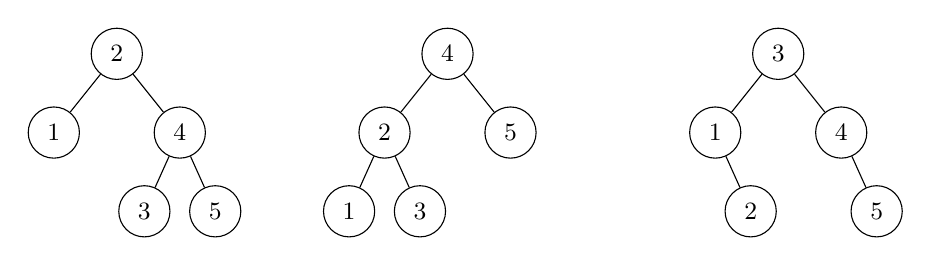
\begin{tikzpicture}[n/.style={circle,draw,inner sep=0pt,minimum size=6.5mm,font=\small},
  level distance=10mm, level 1/.style={sibling distance=16mm}, level 2/.style={sibling distance=9mm}]
\node[n] at (0,0) {2}
  child {node[n] {1}}
  child {node[n] {4} child {node[n] {3}} child {node[n] {5}}};
\node[n] at (4.2,0) {4}
  child {node[n] {2} child {node[n] {1}} child {node[n] {3}}}
  child {node[n] {5}};
\node[n] at (8.4,0) {3}
  child {node[n] {1} child[missing] child {node[n] {2}}}
  child {node[n] {4} child[missing] child {node[n] {5}}};
\end{tikzpicture}
\end{center}
逐一檢查平衡：第一棵，根 2 的左子樹高 $1$、右子樹高 $2$；節點 4 兩邊都高 $1$。 第二棵對稱。 第三棵，
根 3 兩邊都高 $2$；節點 1 左邊高 $0$、右邊高 $1$；節點 4 同樣。 每個節點的高度差都不超過 $1$，而且
中序都是 $1, 2, 3, 4, 5$。

\textbf{㈡} 共 $1 + 1 + 4 = 6$ 種。 根為 3 的四種是左子樹 $\{1, 2\}$、右子樹 $\{4, 5\}$ 各兩種形狀的組合：
\[
3(1(\text{右子 } 2), 4(\text{右子 } 5)),\ 3(1(\text{右子 } 2), 5(\text{左子 } 4)),\
3(2(\text{左子 } 1), 4(\text{右子 } 5)),\ 3(2(\text{左子 } 1), 5(\text{左子 } 4)),
\]
加上根為 2 和根為 4 的各一種。 對照：$5$ 個節點的二元搜尋樹總共有卡特蘭數 $C_5 = 42$ 種，其中只有
$6$ 種是 AVL 樹。
\end{pastsoln}
